\chapter{Network Architectures} \label{appendix:network_architectures}

\begin{figure}[!tbp]
	\centering
    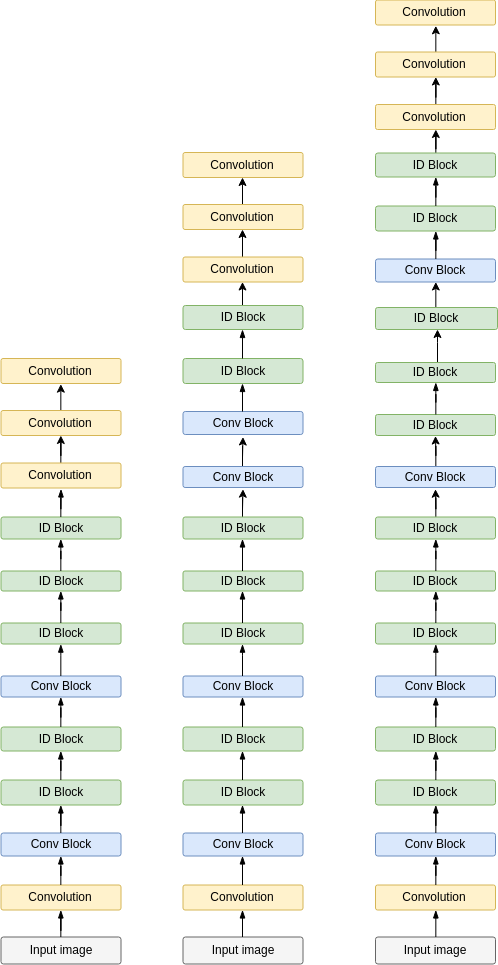
\includegraphics[width=0.7\linewidth]{network_architecture_comparison}
    \caption{The different architectures used in the experiments of Chapter \ref{chapter:experiments}.Architectures 1 and 3 use the leftmost structure with a total of 23 convolutional layers. We constructed architecture 2 using the layout in the middle with 35 layers. Architectures 4, 5 and 6 use the 50 layers structured as shown on the right, although architectures 4 and 6 employ dropout layers with different frequencies after each block and omit the batchnormalization layers. We omitted the batchnormalization layers in the other to structures for displaying purposes.}
    \label{fig:network_architecture_comparison}
\end{figure} 

\chapter{Experiments}